\documentclass[11pt]{article}

\usepackage[a4paper,margin=1in]{geometry}
\usepackage{graphicx}
\usepackage{booktabs}
\usepackage{amsmath}
\usepackage{siunitx}
\usepackage{float}
\usepackage{hyperref}
\usepackage{caption}

\title{HA2 Report: CLIP Zero-Shot Classification on Caltech101}
\author{Your Name}
\date{\today}

\begin{document}
\maketitle

\section{Summary}

This project applies OpenAI CLIP to zero-shot image classification on Caltech101.
The dataset is selected from the CLIP prompt list, and CIFAR10/CIFAR100 are excluded.
We evaluate two CLIP backbones, \texttt{ViT-B/32} and \texttt{ViT-B/16}, under two prompt settings:
a simple single-template baseline and a multi-template ensemble strategy.

The final full run uses all available evaluation samples in torchvision Caltech101
(8,677 images, 101 classes).
Overall, \texttt{ViT-B/16} gains a small accuracy improvement from prompt ensembling,
while \texttt{ViT-B/32} shows a slight drop.
In both cases, McNemar tests indicate that the simple-versus-ensemble difference is not statistically significant at the 0.05 level.

\section{Methodology}

\subsection{Dataset and Label Space}

We use \texttt{torchvision.datasets.Caltech101}.
In this loader, the effective label space contains 101 classes.
Class names are mapped to CLIP prompt labels from the official prompt documentation.

\subsection{Model and Zero-Shot Inference}

We use CLIP models from the official implementation: \texttt{ViT-B/32} and \texttt{ViT-B/16}.
The task is pure zero-shot inference; no parameter fine-tuning is performed.
For each model, image embeddings are computed once and cached.
Text embeddings are generated from prompt templates, then matched to image embeddings by cosine-style similarity.

\subsection{Prompt Settings}

\textbf{Simple template (B1).}
We follow the assignment format exactly:
\begin{quote}
\texttt{a photo of a \{CLASS\}.}
\end{quote}

\textbf{Ensemble template (M1).}
We use all 34 templates provided for Caltech101 in CLIP \texttt{prompts.md}.
Our default aggregation computes template-wise text features and averages them in feature space.

\subsection{Exploration of Effective Ensemble Strategies}

To explore a practical and effective ensemble implementation, we include three ablations:
\begin{itemize}
  \item \textbf{A1 (template count):} $k \in \{1,2,4,8,16,34\}$ with five random seeds.
  \item \textbf{A2 (aggregation):} feature-mean versus logit-mean.
  \item \textbf{A3 (normalization):} normalized versus non-normalized matching.
\end{itemize}

\subsection{Metrics and Statistical Tests}

The primary metric is Top-1 accuracy.
We report bootstrap 95\% confidence intervals and McNemar tests between B1 and M1 for each model.

\section{Results}

\subsection{Main Comparison: Simple vs Ensemble}

Table~\ref{tab:main} reports the main full-run metrics.

\begin{table}[H]
\centering
\caption{Main comparison on full evaluation set.}
\label{tab:main}
\begin{tabular}{lccc}
\toprule
Model & B1 Simple & M1 Ensemble & $\Delta$ (M1-B1) \\
\midrule
ViT-B/16 & 0.8834 & 0.8871 & +0.0037 \\
ViT-B/32 & 0.8759 & 0.8729 & -0.0030 \\
\bottomrule
\end{tabular}
\end{table}

For \texttt{ViT-B/16}, ensembling improves accuracy slightly.
For \texttt{ViT-B/32}, the full 34-template ensemble is slightly worse than the simple baseline.

\begin{figure}[H]
\centering
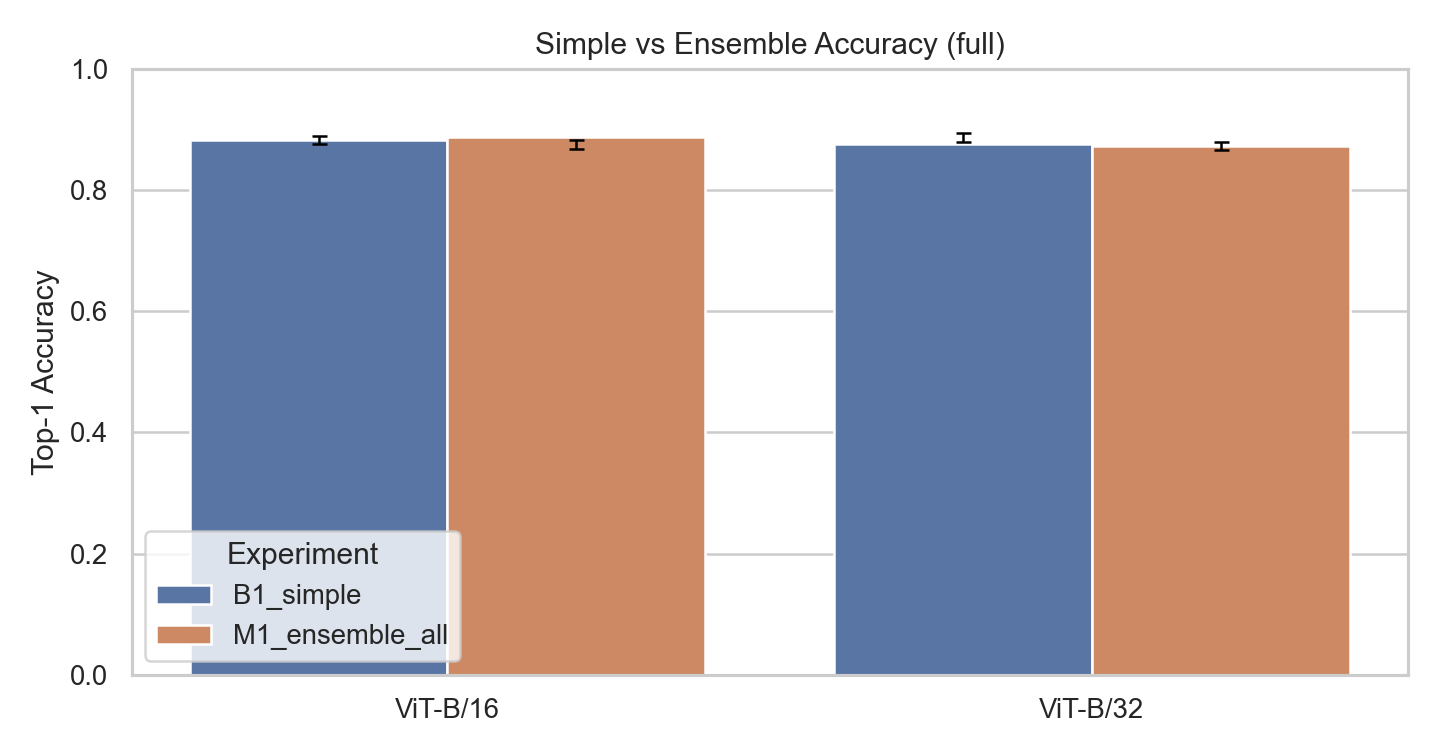
\includegraphics[width=0.78\linewidth]{../artifacts/figures/fig_main_bar_ci_full.png}
\caption{Simple vs ensemble accuracy with bootstrap confidence intervals.}
\label{fig:main}
\end{figure}

The confidence intervals are narrow for both models (around $\pm$0.007 half-width),
which confirms stable estimates under full-data evaluation.

\subsection{Statistical Significance}

McNemar tests compare B1 and M1 on paired predictions:
\begin{itemize}
  \item ViT-B/16: $p = 0.182$
  \item ViT-B/32: $p = 0.315$
\end{itemize}

Both p-values are above 0.05.
Therefore, under this setup, the ensemble effect is small and not statistically significant.

\subsection{Ablations}

\paragraph{A1: template count.}
For \texttt{ViT-B/16}, the best average performance appears around $k=8$ to $k=16$,
and full $k=34$ is not the best point.
For \texttt{ViT-B/32}, increasing template count generally does not help and may slightly reduce accuracy.

\begin{figure}[H]
\centering
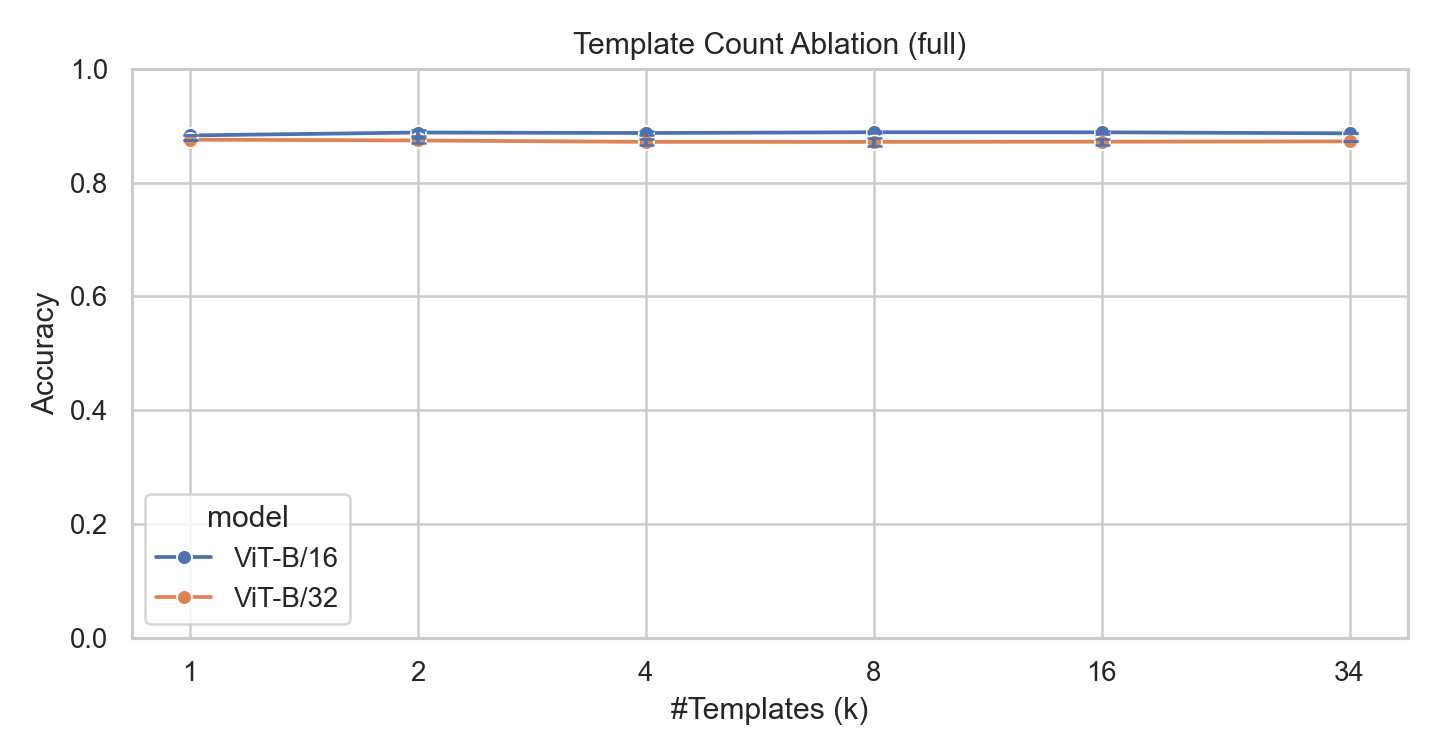
\includegraphics[width=0.78\linewidth]{../artifacts/figures/fig_template_count_curve_full.png}
\caption{A1: accuracy versus template count.}
\label{fig:a1}
\end{figure}

\paragraph{A2: aggregation method.}
\texttt{ViT-B/16} prefers logit-mean (0.8906) over feature-mean (0.8871),
while \texttt{ViT-B/32} prefers feature-mean (0.8729) over logit-mean (0.8668).
This indicates that aggregation choice should be treated as a model-dependent design option.

\paragraph{A3: normalization.}
Normalization is clearly beneficial for both models:
\texttt{norm\_off} drops to about 0.859 for both backbones.

\begin{figure}[H]
\centering
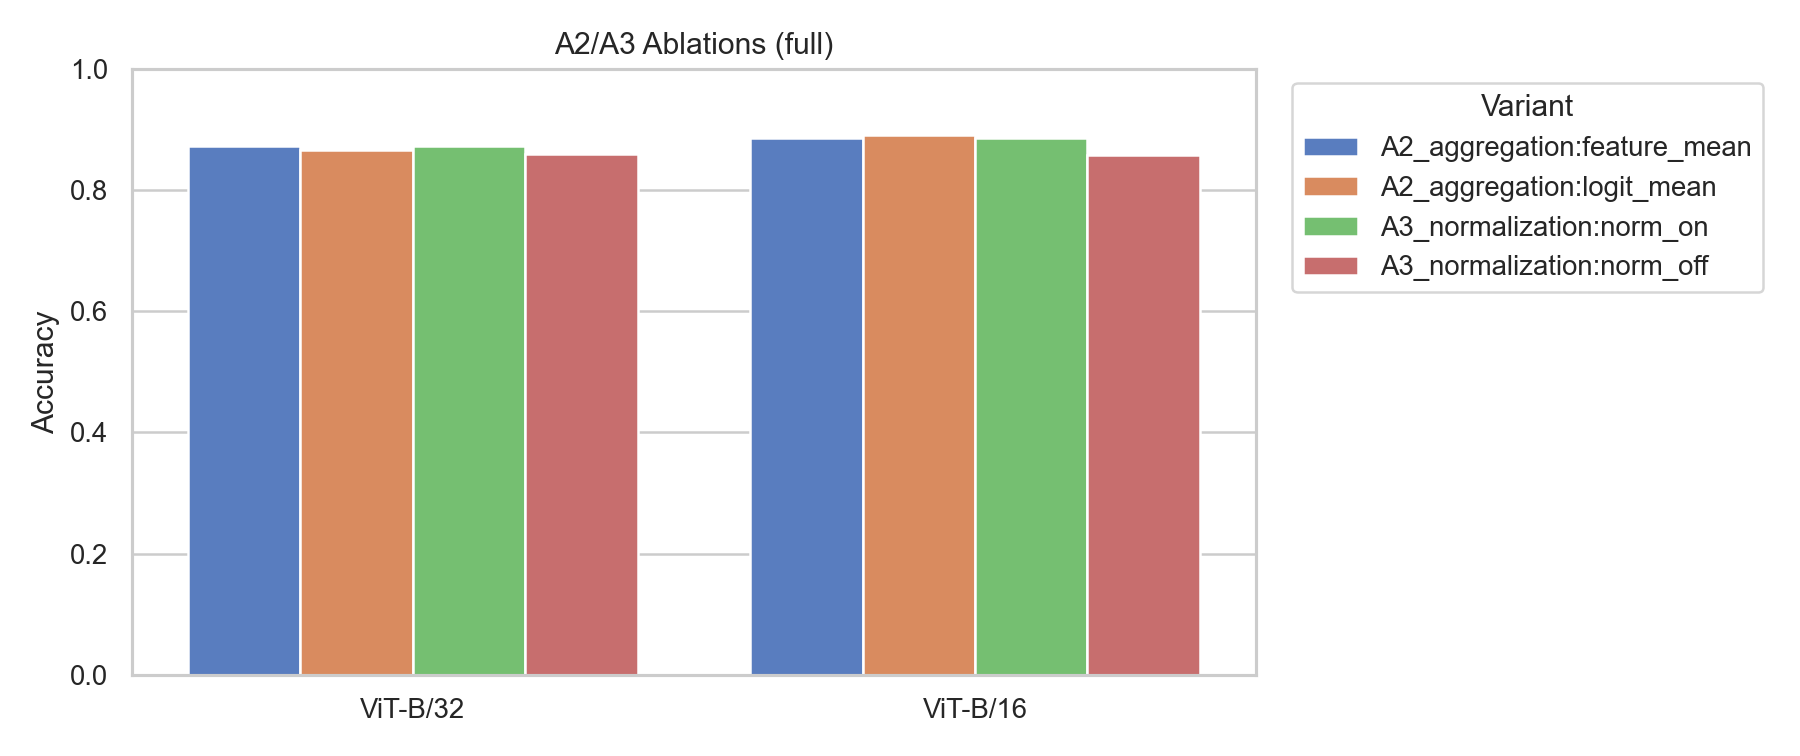
\includegraphics[width=0.82\linewidth]{../artifacts/figures/fig_ablation_grouped_full.png}
\caption{A2 and A3 ablations.}
\label{fig:a23}
\end{figure}

\section{Visualization and Error Analysis}

We inspect frequent confusion pairs and sample-level prediction cases.

\begin{figure}[H]
\centering
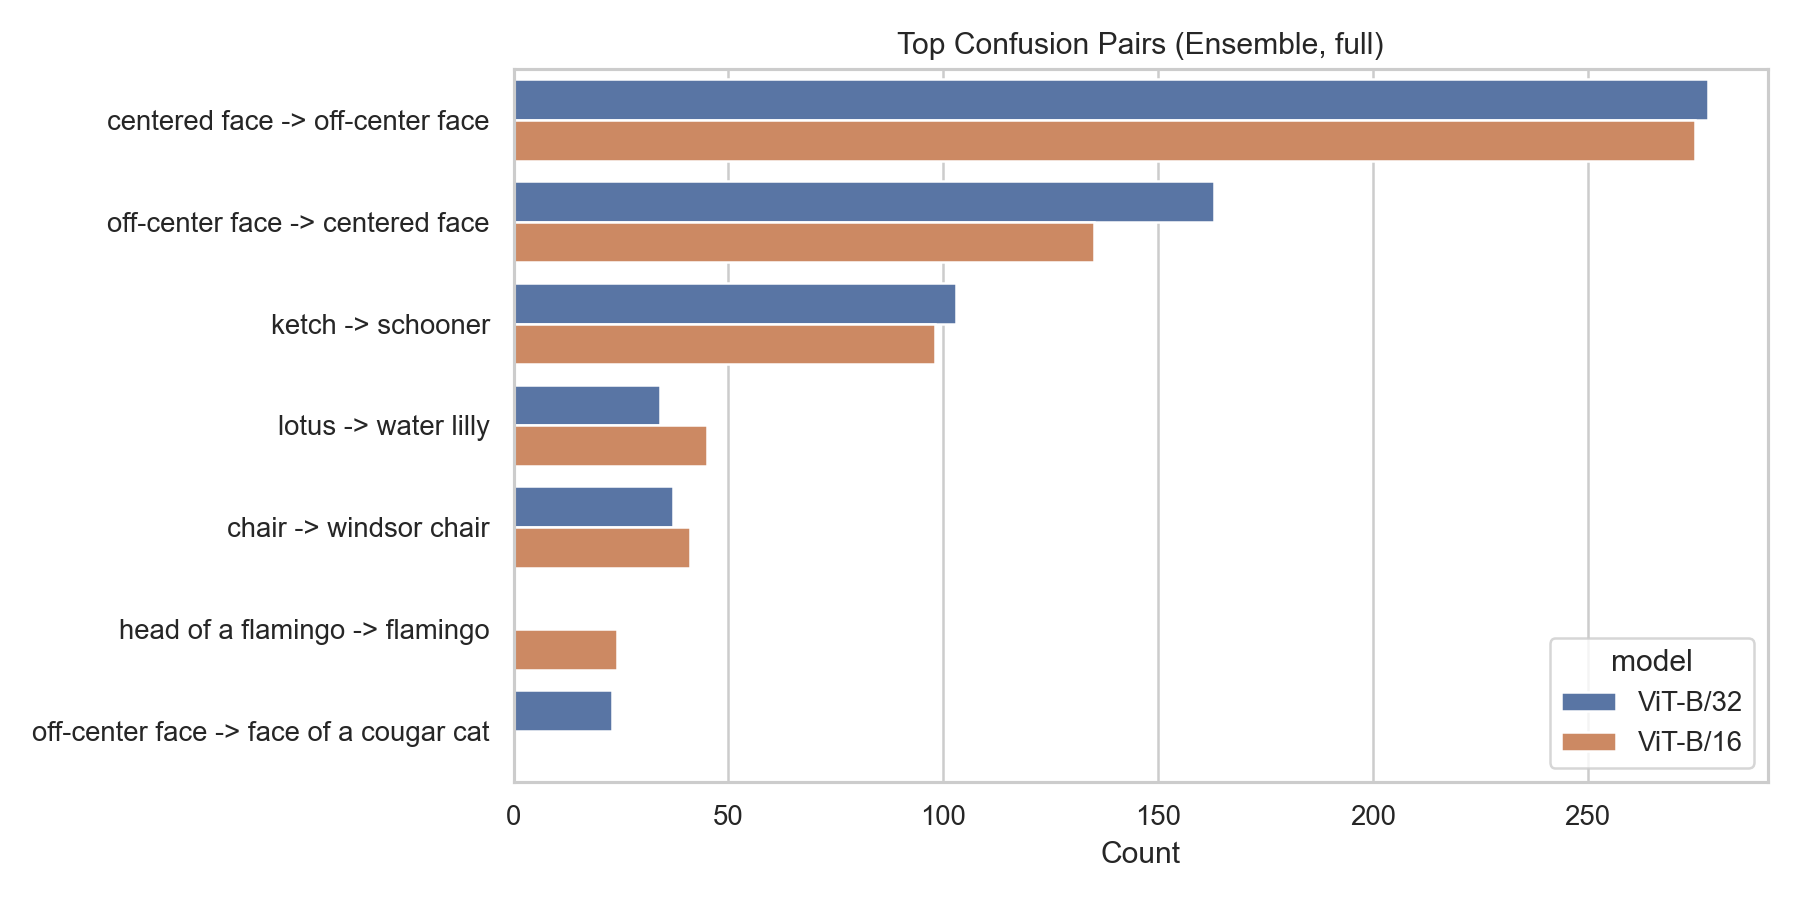
\includegraphics[width=0.84\linewidth]{../artifacts/figures/fig_top_confusions_full.png}
\caption{Top confusion pairs under ensemble predictions.}
\label{fig:conf}
\end{figure}

The most common mistakes are semantically close classes, such as:
\textit{centered face} vs \textit{off-center face}, and \textit{ketch} vs \textit{schooner}.
This pattern is expected in zero-shot settings, where prompt wording and visual granularity both matter.

\begin{figure}[H]
\centering
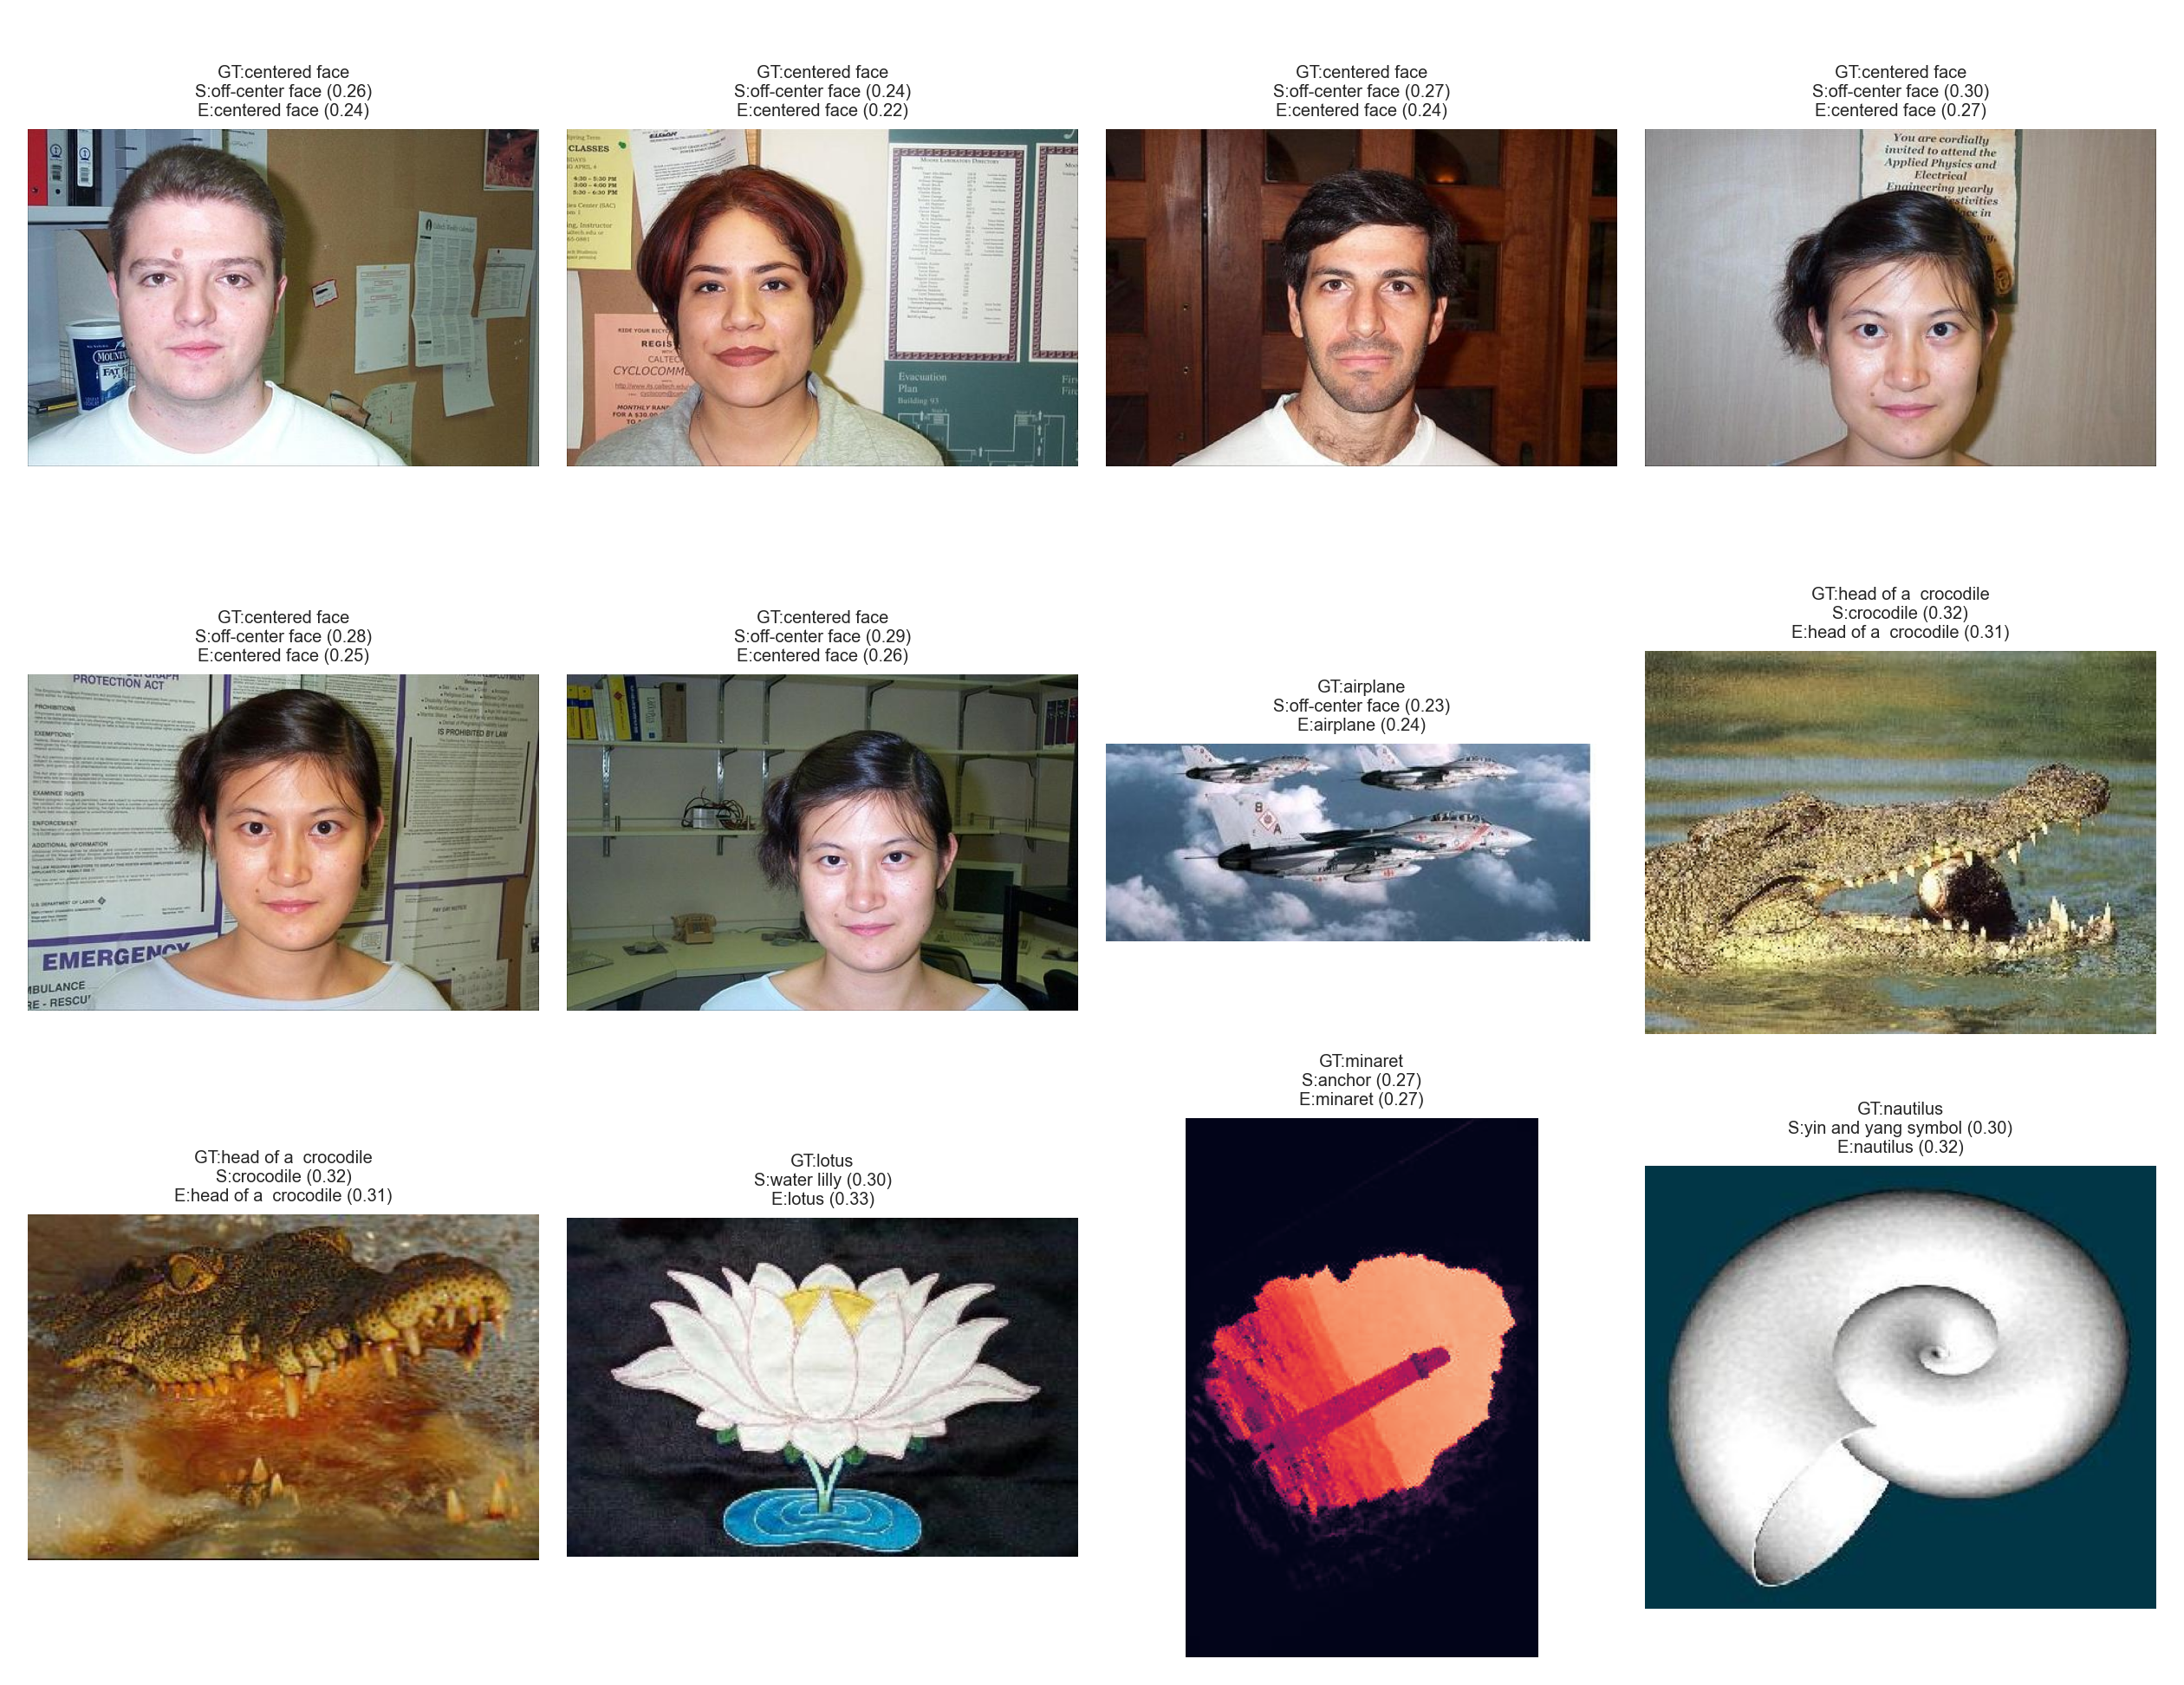
\includegraphics[width=0.96\linewidth]{../artifacts/figures/fig_cases_improved_grid_full.png}
\caption{Examples improved by ensemble prompts.}
\label{fig:improved}
\end{figure}

\begin{figure}[H]
\centering
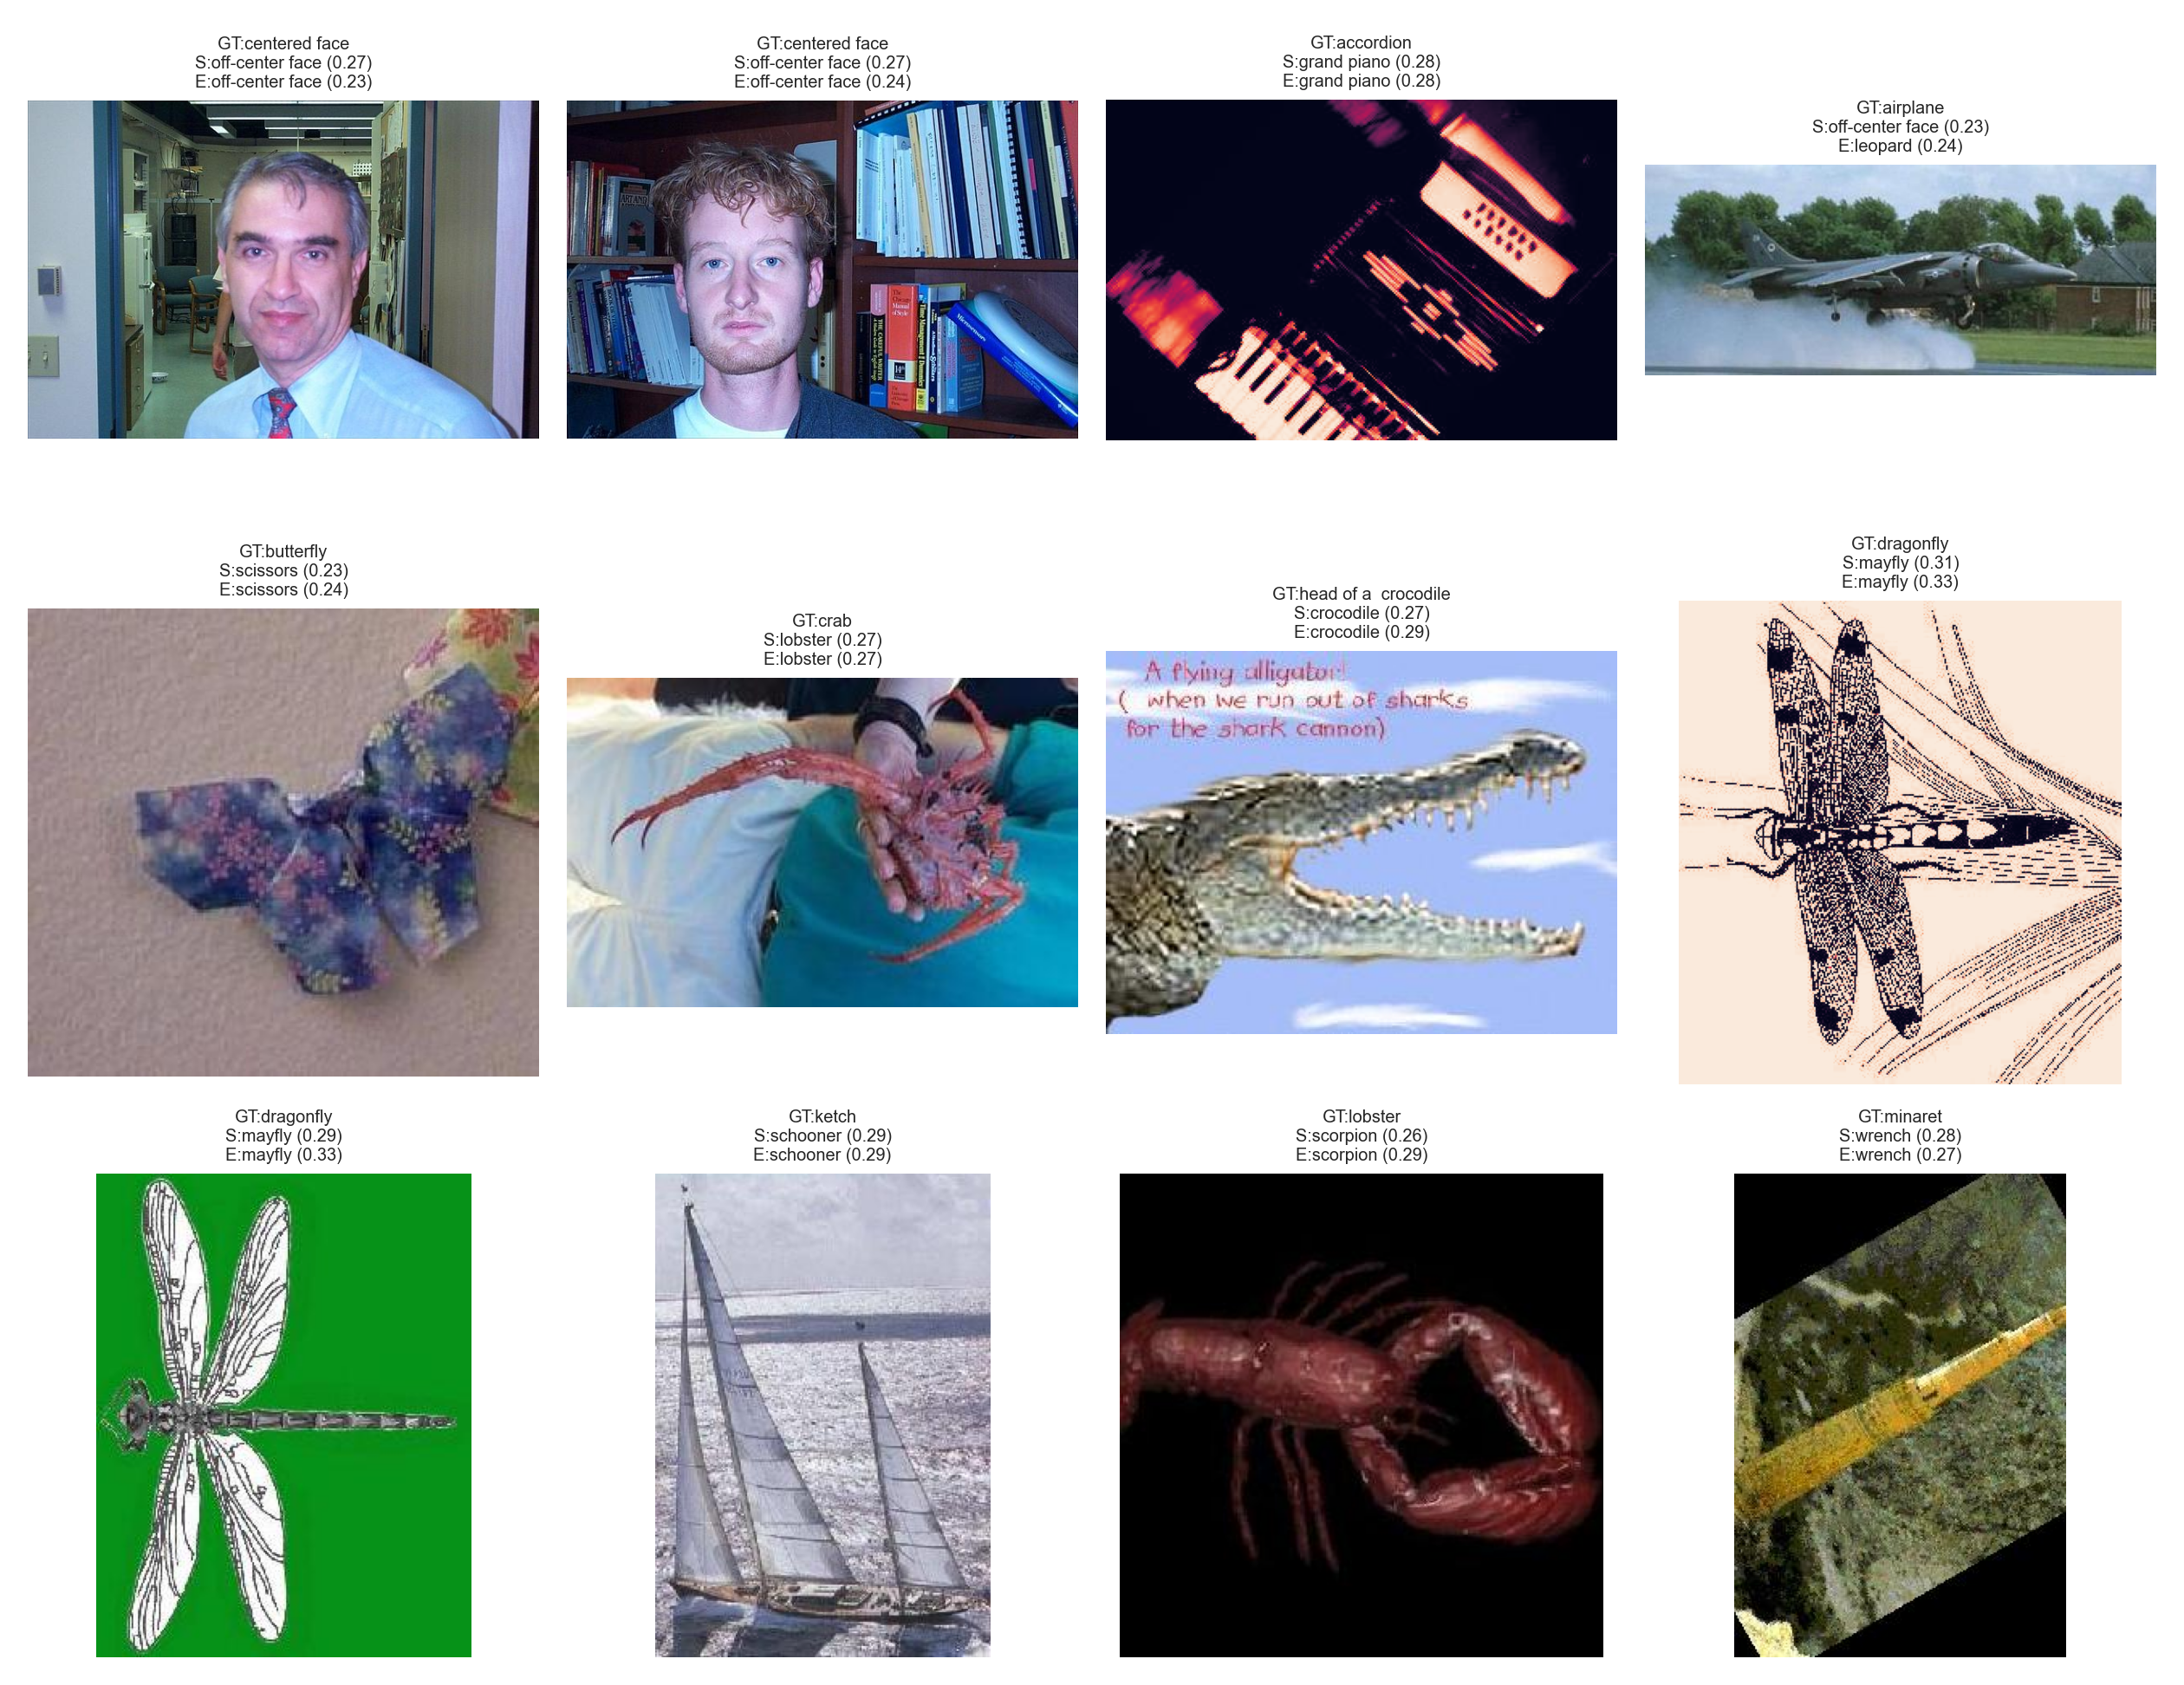
\includegraphics[width=0.96\linewidth]{../artifacts/figures/fig_cases_failed_grid_full.png}
\caption{Examples still misclassified after ensembling.}
\label{fig:failed}
\end{figure}

These examples show that prompt ensembling can fix part of the errors,
but difficult fine-grained cases remain challenging.

\section{Discussion}

The experiments suggest three practical points.
First, using more templates is not always better; moderate template counts can be competitive or better than the full set.
Second, the best aggregation strategy can change by backbone.
Third, embedding normalization is essential for stable performance.

A key limitation is that class-name mapping and template semantics can introduce bias.
Small wording changes may alter decision boundaries in zero-shot inference.
Future work can focus on class-conditional template selection or weighted ensembling rather than uniform averaging.

\section{Conclusion}

This work implements and evaluates CLIP zero-shot classification on Caltech101 with both simple and ensemble prompts.
The final results show a small gain for \texttt{ViT-B/16} and a small drop for \texttt{ViT-B/32} when using all ensemble templates.
Although the average gains are limited in this setting, the ablations provide clear guidance on effective implementation choices,
especially for aggregation design, template count selection, and normalization.

\end{document}
